\documentclass{article}


% if you need to pass options to natbib, use, e.g.:
%     \PassOptionsToPackage{numbers, compress}{natbib}
% before loading neurips_2023


% ready for submission
\usepackage{neurips_2023}


% to compile a preprint version, e.g., for submission to arXiv, add add the
% [preprint] option:
%     \usepackage[preprint]{neurips_2023}


% to compile a camera-ready version, add the [final] option, e.g.:
%     \usepackage[final]{neurips_2023}


% to avoid loading the natbib package, add option nonatbib:
%    \usepackage[nonatbib]{neurips_2023}

\usepackage[utf8]{inputenc} % allow utf-8 input
\usepackage[T1]{fontenc}    % use 8-bit T1 fonts
\usepackage{hyperref}       % hyperlinks
\usepackage{url}            % simple URL typesetting
\usepackage{booktabs}       % professional-quality tables
\usepackage{amsfonts}       % blackboard math symbols
\usepackage{nicefrac}       % compact symbols for 1/2, etc.
\usepackage{microtype}      % microtypography
\usepackage{xcolor}         % colors

\usepackage{amsmath}
\DeclareMathOperator*{\argmax}{\arg\!\max}
\usepackage{float}
\usepackage{graphicx}
\usepackage{subfigure}
\usepackage{parskip}

%My Macros
\newfont{\msym}{msbm10}
\newcommand{\reals}{\mbox{\msym R}}


\title{Seeking agreement\\ {\large an ensemble approach to epistemic uncertainty} }


% The \author macro works with any number of authors. There are two commands
% used to separate the names and addresses of multiple authors: \And and \AND.
%
% Using \And between authors leaves it to LaTeX to determine where to break the
% lines. Using \AND forces a line break at that point. So, if LaTeX puts 3 of 4
% authors names on the first line, and the last on the second line, try using
% \AND instead of \And before the third author name.


\author{%
  David S.~Hippocampus\thanks{Use footnote for providing further information
    about author (webpage, alternative address)---\emph{not} for acknowledging
    funding agencies.} \\
  Department of Computer Science\\
  Cranberry-Lemon University\\
  Pittsburgh, PA 15213 \\
  \texttt{hippo@cs.cranberry-lemon.edu} \\
  % examples of more authors
  % \And
  % Coauthor \\
  % Affiliation \\
  % Address \\
  % \texttt{email} \\
  % \AND
  % Coauthor \\
  % Affiliation \\
  % Address \\
  % \texttt{email} \\
  % \And
  % Coauthor \\
  % Affiliation \\
  % Address \\
  % \texttt{email} \\
  % \And
  % Coauthor \\
  % Affiliation \\
  % Address \\
  % \texttt{email} \\
}


\begin{document}
\nolinenumbers'

\maketitle


\begin{abstract}
  The abstract paragraph should be indented \nicefrac{1}{2}~inch (3~picas) on
  both the left- and right-hand margins. Use 10~point type, with a vertical
  spacing (leading) of 11~points.  The word \textbf{Abstract} must be centered,
  bold, and in point size 12. Two line spaces precede the abstract. The abstract
  must be limited to one paragraph.
\end{abstract}


\section{Introduction}
Quantifying prediction uncertainty is an active area of research in
machine learning and
elsewhere~\cite{breiman1993fitting,li2008knows,hora1996aleatory,mc-dropout,der2009aleatory,hullermeier2019aleatoric}. A
useful way to reason about uncertainty is to divide it into {\em
  aleatoric} vs {\em epistemic} uncertainty.We demonstrate this
partition by considering our model to be a DNN for binary
classification.  We consider a single example $x$ our goal is to
preict the associated label $y \in \{-1,+1\}$.


Suppose the learned
prediction function $f$ (the weights of the NN) is a fixed function
$f: X \to \reals$. The aleatoric, ot intrinsic uncertainty is captured
by the conditional probability $p_a=P(y=+1|f(x)>a)$. This so-called
``calibration function'' is ``intrinsic'' because it does not depend
on the training set.

On the other hand the epistemic uncertainty orresponds to {\em model uncertainty} i.e. the uncertainty the we have in the model



knowledge as to which function $f$ is best. 


divide prediction uncertainty is to divide preidction uncertainty it into
aleatory vs. epistemic uncertainties. We briefly describe what this
means in the context of binary classification using a NN. Denote a
binary example by $(x,y)$. Let $M$ 





useful way to distinguish between different types of uncertainty is to
differentiate aleatory or irreducible uncertainty from epistemological
or reducible uncertainty. Consider predicting the outcome of flipping
a coin whose (unknown) probability of heads is $p=1/4$. If we know $p$
we should always predict ``tails'' and will be incorrect with
probability $1/4$. This uncertainty is irreducible, because no amount
of additional data will change it. On the other hand, if we flip the
coin $n$ times and find that $m$ of the outcomes were ``heads'' we can
estimate the true value of $p$ to be approximately
$\frac{m}{n} \pm \frac{1}{\sqrt{n}}$. The range
$\pm \frac{1}{\sqrt{n}}$ is the epistemological or reduxible
uncertainty, because it relates to our {\em knowledge} regarding $p$
which can be improved by increasing $n$.

In this paper we show how epistemological uncertainty in DNN can be reduced using a simpl ensemble based method. Our approach is based on projecting the model uncrtainty onto instances and measuring the resulting per-nstance uncertainty.

{\bf Yoav} till here.


Modern DNN have increasingly complex architectures involving tens of millions of parameters. Experience shows that increasing the depth and width of the DNN generally leads to better performance. The question we ask is whether increasing the number of parameters is equally important for every test example. We carried some experiments using CIFAR-10. Not surprisingly, we find that different examples require different levels of complexity. 

What {\em is} surprising, however, is the fact that for {\em most} examples a very simple network suffices, only a small fraction of the examples benefits from complex networks. We call examples of the first type {\em easy} and those of the second type {\em hard}. our results suggest that the hardness of an example is an {\em inherent} property of the example and depends only weakly on the type and architecture of the network.

Prior work on this subject~\cite{} is based on the amount of training required to get the example labeled correctly. The problem with this measure is that it requires knowing the correct label and therefor cannot be used at test time. We suggest an ensemble-based approach to measure hardness that does not require knowing the true label.


\section{Related Work}
\cite{stacked_ovr}introduced a framework to deal with multiclass classification task in a one-vs-rest(OVR) way, which is similar to ours that treat each 10-class classification task as 10 binary classification tasks. It also trains multiple classifiers. However, its classifiers are not independent and they work in a stacked order and each classifier is responsible for one class. This paper also pay attention to easy classes and confusing classes and it uses the classes’ easiness to arrange the order of the classifiers.
The key differences to our work are(Need further verify, I haven’t carefully read the details yet): (1)It need labels to define the confusing classes. (2)Whether an example is confusing only matters in the training stage, it no longer cares if it’s confusing in the inferencing stage.

\cite{deephash} focus on building hash for images to make search and retrieve of the images efficient. And it pay attention to the easy and hard examples. However, it needs labels to tell which one is easy or hard. And it only focus on the easiness on training process.

\cite{focal_loss} This paper mentioned a concept: Focal Loss(Not originated in this paper). It also focus on the uncertainty of the classifier’s prediction. But simply using the difference between the predicted score and ground truth as the measure of uncertainty which is very different from ours.

I will look for more paper focusing on easy-confusing examples. Till now, I find most works that pay attention to the easiness and confusion of examples are only trying to make use of it in the training stage to improve the training process. After they get the trained framework, they no longer care about whether an example is easy or confusing on the inference stage, but to simply predict a label in the classical way. But our framework can distinguishing the hardness of the examples on the inference stage, and is able to tell the uncertainty quantitatively.

\begin{itemize}
  \item \cite{mc-dropout}: Add dropout in the inference stage. This can generate an 'ensemble' without really training multiple predictors. However, this paper doesn't propose novel ways to make use of the ensemble outputs. Actually the mc-dropout method can be combined with ours.
  \item \cite{deep-ensemble} It does three things: (1) Directly predict uncertainty as part of the predictor output(i.e, the predictor's output should be a normal distribution with mean value and uncertainty rather than just a single value) and properly add this uncertainty into the loss function. (2)Use adversarial training (3)Train an ensemble to estimate the predicted mean value and uncertainty. Difference to ours: (1)The way to make use of the ensemble output is different from us: treat the ensemble as a uniformly-weighted gaussian mixture. (2)Doesn't mention predicting a SET.
  \item \cite{selective-classification} Constructs a method to find a proper threshold for confidence-rate(Can be almost any function) so that only the confident predictions will be made(Say don't know for unconfident). Difference to ours: (1)doesn't use ensemble(The author mentioned ensemble saying using ensemble costs too much). (2) Doesn't mention predicting a SET.  Seems its way to choose threshold can be applied to our method. We can compare our results with this by regarding the Set size $\neq$ 1 as 'don't know'.
  \item \cite{bias-reduced-uncertainty} Following the work in \cite{selective-classification}, this paper trys to find a good method to measure the confidence-rate. It also uses an ensemble, but the members in the ensemble are not trained independently but rather predictors obtained in different epochs in the training process.
  \item \cite{selectivenet} Designed a way to train predictors that output uncertainty directly. Neither use ensemble nor mention prediction set. We can compare our results with this by regarding the Set size $\neq$ 1 as 'don't know'.
\end{itemize}

\section{Theory}

Many learning algorithms are based on finding the single best
rule. Ensemble methods such as Bagging and Random Forests are based on
combining many rules, each of which is close to
otimal. Averaging/voting across the rules results in a more stable and
more accurate rule.  We use a similar logic for classsification with
one important twist: when the ratio between +1 and -1 predictions is
close to 50\%/50\% our combination rule outputs 0, which can be
interpreted as ``I don't know'' (IDK).

Figure~\ref{fig:duality} is a sketch of ensemble based classification.
The central assumption is that models that are in the close the best
model, in terms of the probability of disagreement, are almost as
accurate as the best model.  models. This implies that under slightly
different training conditions that sub-optimal model can become the
best. We call this set of models the ``support set'' and divide the
instance space into the ``easy'' instances, on which all models in the
support set agree. The ``hard'' instances are those that are not
``easy''. The ``hardness'' of hard examples is measured by the the
difference between the probability~\footnote{Assuming some fixed prior
  distribution.} of the two parts to which the instance divides the
sample.

An ensamble is a sample from the support set. Procedurally, it is generated by
perturbing the training process. In this paper we consider three ways of perturbing the training process, a few more possibilities are listed in the conclusions.
\begin{enumerate}
\item {\bf Bootstrap} perturb the training process by selecting from the size $n$ training set a new training set of size $n$ by sampling from the $n$ times with replacement.
\item{\bf Random starting point} Choose the starting point for gradient descent multiple times independently at random.
\item{\bf Architecture} Choose a different architecture for each ensemble member.
\end{enumerate}

We divide our discussion to the 
We use the binary classification problem as a building block of our solution for multi-label prediction.

\begin{figure}[tbh]
    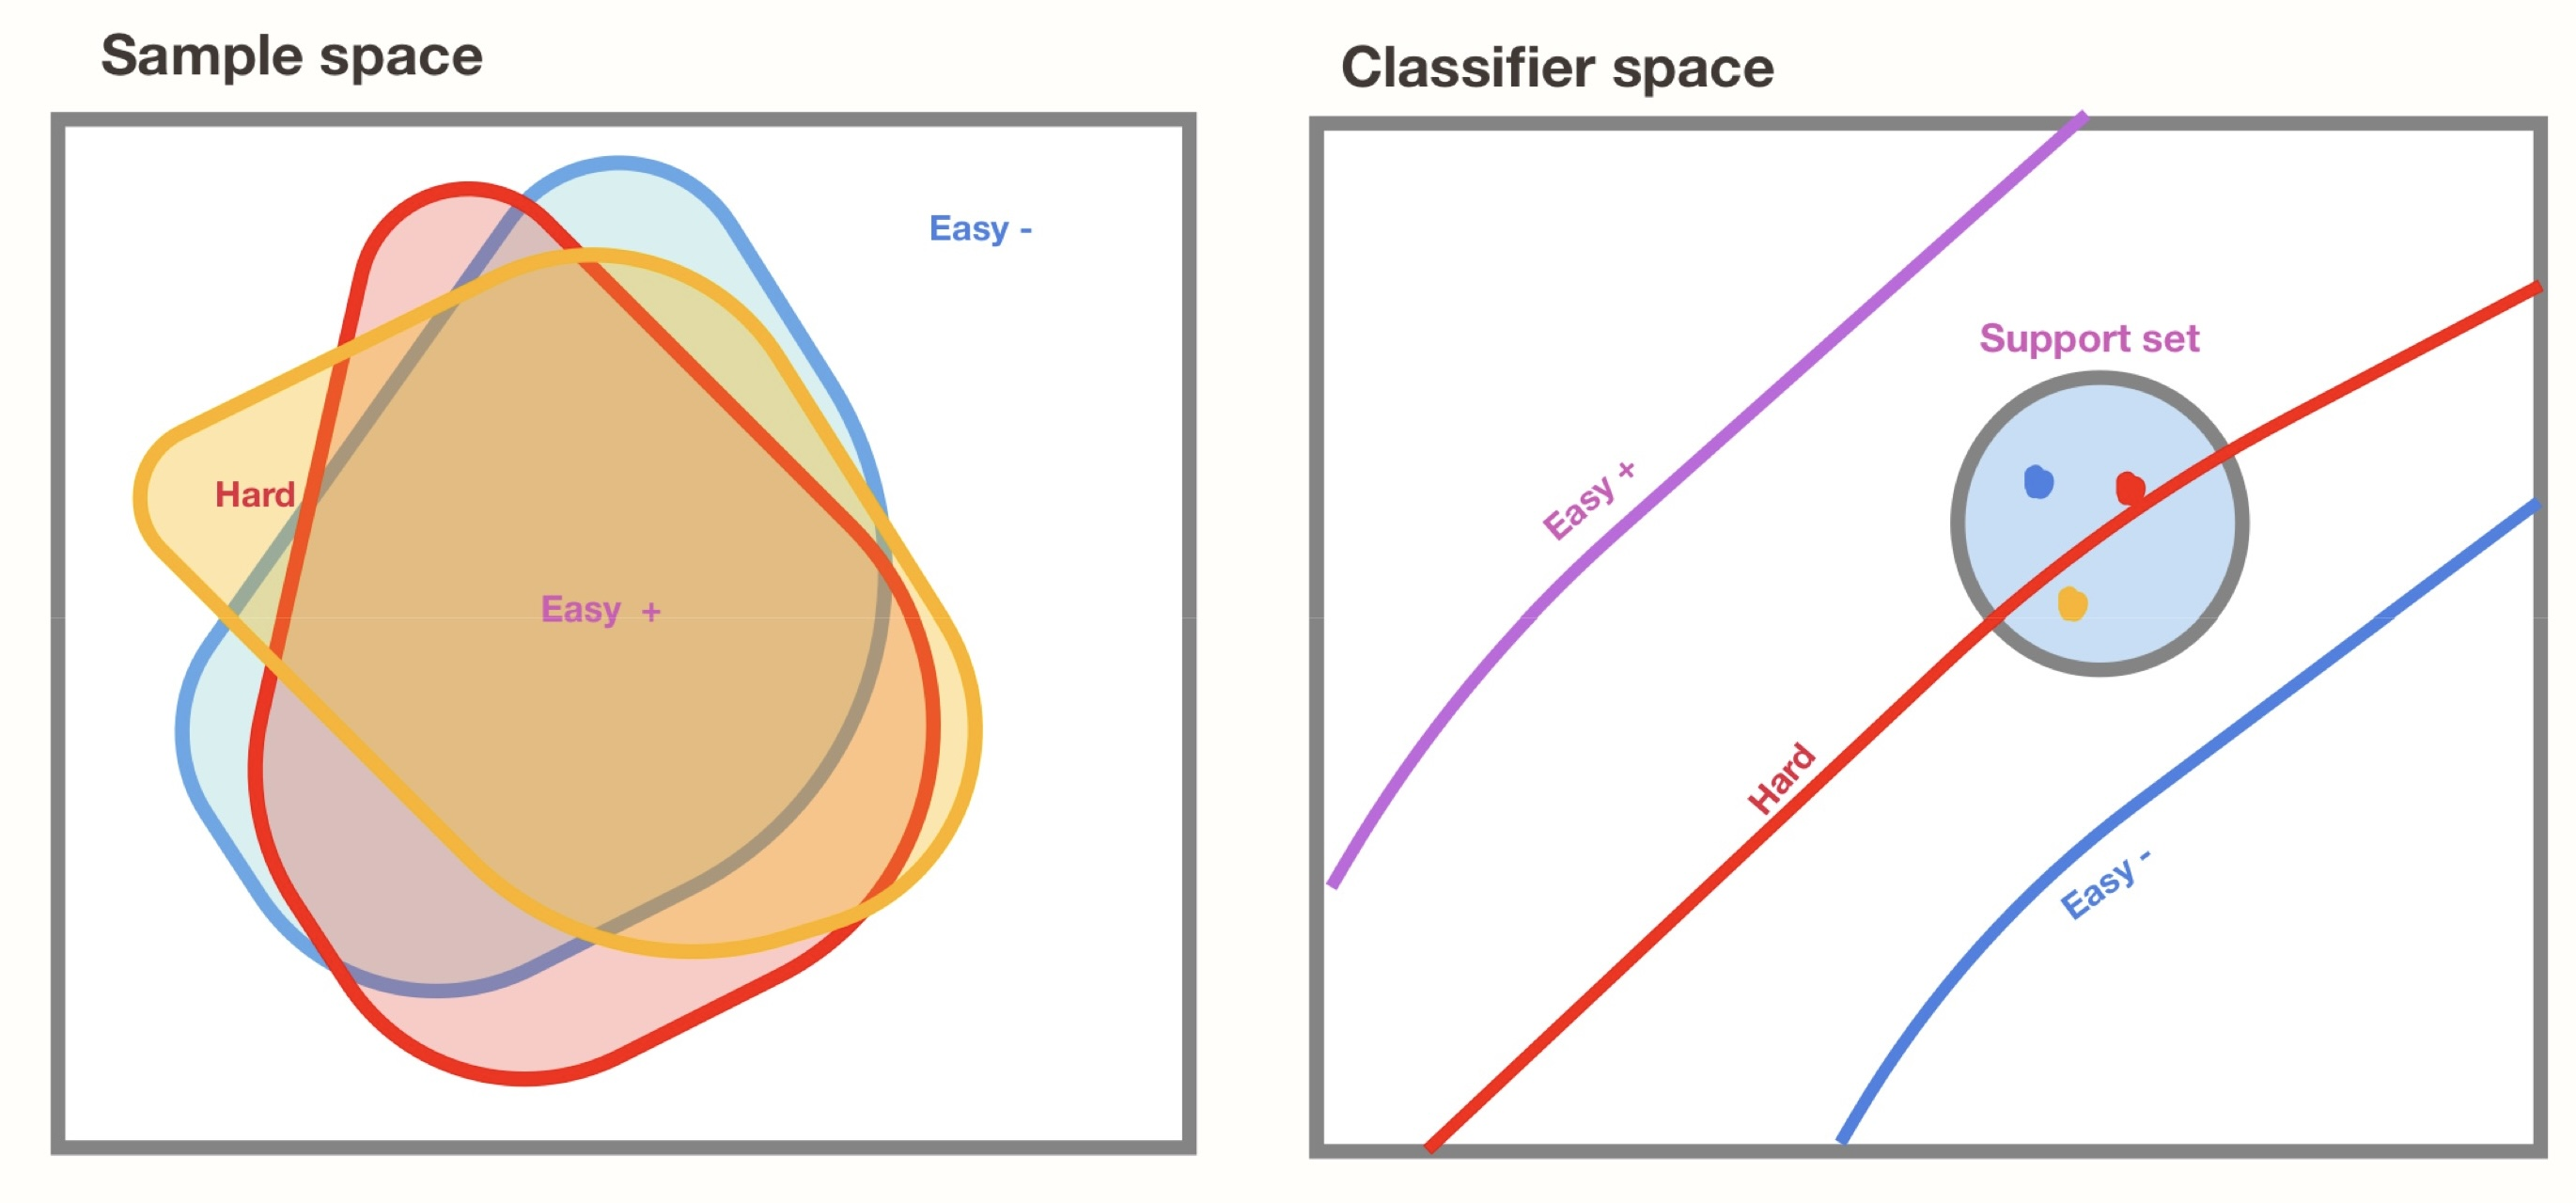
\includegraphics[width=\textwidth]{figs/SupportSet.jpg}
\label{fig:struc}
\caption{\textbf{Duality between classifiers and examples} Each point
  in the sample space figure corresponds to a sample, the three shaded
  sets correspponds to an ensemble of 3 classification rules with
  similar training error. ``Easy -'' is an instance on which the
  ensemble predicts unanimously ``-'', while ``Easy+'' is an instance
  on which the unanimous prediction is ``+''. It is this unanimity
  that makes the instance ``easy''. The hard instance is one on which
  classifiers disagree.  The classifier space (parameter space),
  demonstrates the same relationships between instances and
  classifiers, but here each classifier is a point and the instances
  define boundaries between classifiers that predict ``+' or ``-'' on
  the instance. THe {\em support set} is the set of classifiers whose
  performance is close to optimal. The three dots correspond to the
  ensemble of three classifiers. Finally, easy instances are ones on
  which the rules in the support set are unanimous, while the hard
  example splits the support set in two. \label{fig:duality}}
\end{figure}


\subsection{Binary Case}
In a standard binary classification task, given an input $\textbf{x}$,
the predictor will output either $+1$ or $-1$. In our framework the
model can predict $0$ in addition to $-1$ and $+1$, where $0$ stands
for ``hard instance'' or ``I don't know the label''.

To quantify


e don't use the binary classification or the logit value generate from the score, instad, we use the score by a DNN.


Usually in a binary classification task, a neural networks predictor calculates a real value. In the training stage this value can be further transfered by a sigmoid funtion to a real value ranging from 0 to 1 and then pluged into the loss function; while in the inferencing stage, this value can be compared with 0 to decide whether this example belongs to the positive class or the negative class. Denote this value calculated by predictor $f \left(\cdot , \mathcal{P}\right)$ as $O_f \left(\cdot , \mathcal{P}\right)$. If $O_f \left(x , \mathcal{P}\right)$ is larger than 0, the example will be classified into the positive class, otherwise the negative class.

\textit{\textbf{Assumption}} As we change the pertubation $\mathcal{P}$ to get $O_f \left(x , \mathcal{P}_1\right)$, $O_f \left(x , \mathcal{P}_2\right)$,$\cdots$, $O_f \left(x , \mathcal{P}_i\right)$,$\cdots$,$O_f \left(x , \mathcal{P}_E\right) $, the values $O_f \left(x , \mathcal{P}_i\right)$ obeys a normal distribution $\mathcal{N}(\mu,{\sigma}^2)$. 

The mean value $\mu$ should be positive if this example belongs to the positive class and negative if it belongs to the negative class. After training an ensemble $f \left(\cdot , \mathcal{P}_1\right), f \left(\cdot , \mathcal{P}_2\right),\cdots, f \left(\cdot , \mathcal{P}_i\right),\cdots,f \left(\cdot , \mathcal{P}_E\right) $, we can esitimate how confident we are to say $\mu$ is positive or negative based on $O_f \left(x , \mathcal{P}_1\right), O_f \left(x , \mathcal{P}_2\right),\cdots, O_f \left(x , \mathcal{P}_i\right),\cdots,O_f \left(x , \mathcal{P}_E\right) $. This can be done by \textit{t-test}. The null hypothesis is $\mu = 0$, and the \textit{t}-statistic is: 

\begin{equation}
    t = \frac{\overline{O}_f\left(x , \mathcal{P}\right)}{S/\sqrt{E}}
\end{equation}

where
    \begin{eqnarray}
            \overline{O}_f\left(x , \mathcal{P}\right) &= \frac{1}{E} \sum_{i=1}^E O_f\left(x , \mathcal{P}_i\right) \\
            S^2 &= \frac{1}{E-1} \sum_{i=1}^E {(O_f\left(x , \mathcal{P}_i\right) - \overline{O}_f\left(x , \mathcal{P}\right))}^2
    \end{eqnarray}

denote the $\textit{p}$-value of the test as $\textit{p}$, we define our confidence as:
\begin{equation}
    confidence = -sign( \overline{O}_f\left(x , \mathcal{P}\right))*log(\textit{p})
\end{equation}

If the predictors are very confident that the example belongs to the positive class, the confidence should be a very large positive value; if the predictors are confident of the negtatice class, it should be a very small negative value. If the predictors are unsure, the confidence value would be close to 0. We can set a threshold to discriminate class+ and class-. Further, with this confidence value, we can set one threshold for confidence class+ and another thereshold for confident class-. In the regime between the two thresholds, the predictors will say "I don't know".

\subsection{Multiclass Case}\label{sec:multi}
In a multiclass classification task, $ \textbf{O}_f \left(x , \mathcal{P}\right)$ is no longer a real value but a $R^C$ vector, $C$ is the number of classes. In the training stage, a softmax can be operated on $ \textbf{O}_f $ and further used in the loss function. In the inferencing stage, $\max_{j} \textbf{O}_{f,i}$ will be taken as the final prediction result, where $\textbf{O}_{f,j}$ refers to the $j$th dimension of the $ \textbf{O}_f $ vector.

To apply our \textit{t-test}-based method, we take each multiclass classification task as multiple binary classification tasks. Based on $\textbf{O}_{f,j} \left(x , \mathcal{P}_1\right),\cdots, \textbf{O}_{f,j} \left(x , \mathcal{P}_i\right),\cdots,\textbf{O}_{f,j} \left(x , \mathcal{P}_E\right) $, we can calculate the \textit{t}-statistic $\textit{t}_j$ and get the \textit{p}-value $\textit{p}_j$ and finally the confidence value $\textit{confidence}_j$ for class $j$. 

We can have different ways to make use of the confidence values, for example:
\begin{enumerate}
    \item The class with the largest confident value will be the predicted class.
    \item Instead of predicting one class, the class with the largest confident value and classes whose confidence is no smaller than the largest by a certain amount will form a prediction set.
    \item We can set a threshold as in the binary case. If $\textit{confidence}_j$ is smaller than the threshold, then the example doesn't belong to class j, otherwise the predictors think the example belongs to class j. Similarly, we can set two thresholds for confident of class j, confident not class j and "I don't know".
\end{enumerate}

The second and the third ways bring a problem: the example may belong to multiple classes or none of the classes. When this happens, it suggests that this example is a "hard" example, because it makes the predictors confused among these classes. The experiment section shows that this confusion indeed happens for human. Therefore, it can be benifit to allow the predictors to say that they are confused and further careful actions are needed to make a decision(For example, call stronger predictors to classify the example), rather than simply give a prediction without confidence. 


Let $\mathcal{D}$ be a dataset containing $\left\{\left( \textbf{x}_i ,y_i\right)\right\}_{i=1}^N $,where $\textbf{x}$ is the oberserved feature vector, $y$ is the label in a classification task or a numerical value in a regression task. For a predictor with a specific architecture $f$ (For example, a ResNet),we can apply a pertubation $\mathcal{P}$ in the training process of $f$ and get a predictor $f \left(\cdot , \mathcal{P}\right)$. When a new observed feature vector $textbf{x}$ comes, the predictor gives a prediction $f \left(\textbf{x} , \mathcal{P}\right)$. Since there are many different kinds of predictors, we can also train a set of predictors with different architectures $f_1,f_2,\cdots,f_i,\cdots,f_K$

\begin{figure}[H]
    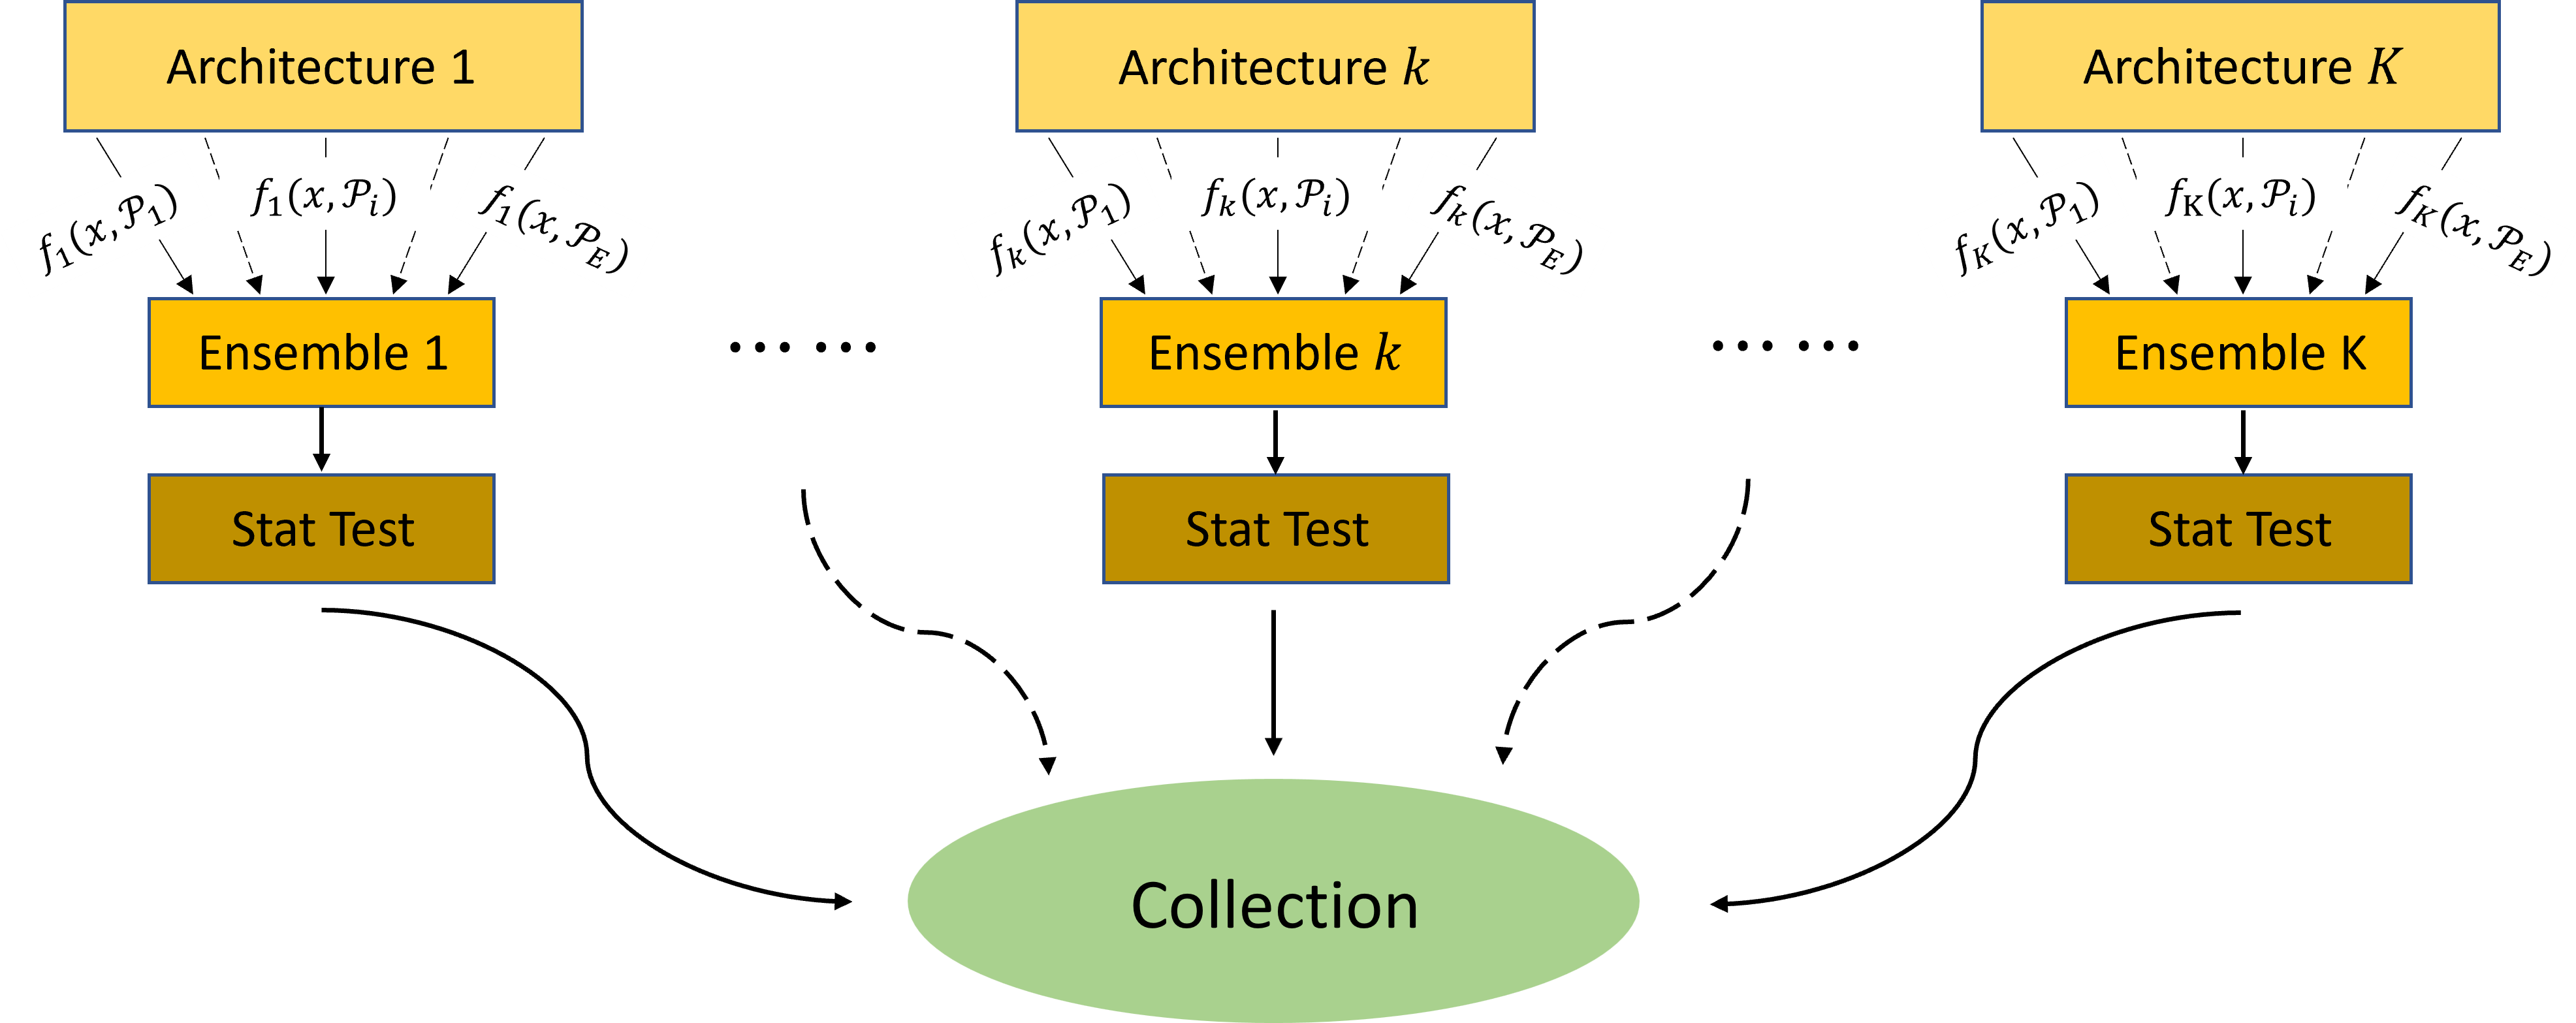
\includegraphics[width=\textwidth]{figs/overall_structure.png}
\label{fig:struc}
\caption{\textbf{Structure of Our Framework}}
\end{figure}

\subsection{Three types of Pertubations: BootStrap, Architecture Starting Points and Architecture }
There are two common ways to pertubate the training process:

\textit{\textbf{Bootstrap}} We can construct a training set $\mathcal{T}$ by randomly draw $M$ examples $\left\{\left( \textbf{x}_i ,y_i\right)\right\}_{i=1}^M $ from $\mathcal{D}$ with replacement. We can sample a set a $\mathcal{T}_1,\mathcal{T}_2,\cdots,\mathcal{T}_i,\cdots,\mathcal{T}_E$ independently, and train a $f$ on each of the training set.
This will generate a set of predictors $f \left(\cdot , \mathcal{T}_1\right), f \left(\cdot , \mathcal{T}_2\right),\cdots, f \left(\cdot , \mathcal{T}_i\right),\cdots,f \left(\cdot , \mathcal{T}_E\right) $ with the same architecture but different parameters.

\textit{\textbf{Random Starting Point}} We take the entire dataset $\mathcal{D}$ as the training set, yet change the initialization of the paremeters in the architecture $f$(For example, use different random seeds to initialize the neural networks). With different starting points $\mathcal{S}_1,\mathcal{S}_2,\cdots,\mathcal{S}_i,\cdots,\mathcal{S}_E$ of the parameters, we can train a set of predictors $f \left(\cdot , \mathcal{S}_1\right), f \left(\cdot , \mathcal{S}_2\right),\cdots, f \left(\cdot , \mathcal{S}_i\right),\cdots,f \left(\cdot , \mathcal{S}_E\right) $



\subsection{Why Ensemble Works}
This section is the analysis of why the aggregation of the ensemble works better than a single predictor.
\subsubsection{For Regression Tasks}
In regression, a common aggregation method is to calculate the average of the ensemble outputs known as \textit{Bagging}, which is:

\begin{equation}
    f^A\left(x\right) = \frac{1}{E}\sum_{i=1}^{E} f\left(x,\mathcal{P}_i\right)
\end{equation}

as $E\rightarrow\infty$, we have:
\begin{equation}
    f^{A*}\left(x\right) = \mathcal{E}_\mathcal{P}\left[f\left(x,\mathcal{P}\right)\right]
\end{equation}

The expectation of the squared error for a single model is:
\begin{equation}
\begin{split}
    \mathcal{E}_\mathcal{P}\left[{\left(y-f \left(\textbf{x} , \mathcal{P}\right)\right)}^2\right] &= y^2 - 2y\mathcal{E}_\mathcal{P}\left[f\left(x,\mathcal{P}\right)\right] + \mathcal{E}_\mathcal{P}\left[f^2\left(x,\mathcal{P}\right)\right] \\
    &= y^2 - 2y\mathcal{E}_\mathcal{P}\left[f\left(x,\mathcal{P}\right)\right] + \mathcal{E}^2_\mathcal{P}\left[f\left(x,\mathcal{P}\right)\right]+\mathcal{E}_\mathcal{P}\left[f^2\left(x,\mathcal{P}\right)\right]-\mathcal{E}^2_\mathcal{P}\left[f\left(x,\mathcal{P}\right)\right] \\
    &= {\left(y-\mathcal{E}_\mathcal{P}\left[f\left(x,\mathcal{P}\right)\right]\right)}^2+\mathcal{E}_\mathcal{P}\left[f^2\left(x,\mathcal{P}\right)\right]-\mathcal{E}^2_\mathcal{P}\left[f\left(x,\mathcal{P}\right)\right] \\
    &= {\left(y-f^{A*}\left(x\right)\right)}^2 + Var\left(f\left(x,\mathcal{P}\right)\right)
\end{split}
\label{equ1}
\end{equation}

The equation \ref{equ1} shows that the expectation of the squared error for a single predictor is larger than the squared error of the aggregation. And the difference is just the variance of the predictor outputs over the pertubation.

\subsubsection{For Classification Tasks}
Assume we have $C$ classes in a classification task, for a given $\textbf{x}$, use $P(j|\textbf{x})$ to denote the "Ground Truth" probability that $\textbf{x}$ belongs to class $j$, we will further discuss what the "Ground Truth" means in later section, here let's just simply take it as the true probability.
Given an input $\textbf{x}$, a single predictor will give a prediction among classes ${1,2,\cdots,j,\cdots,C}$. With an ensemble, we can measure how often the predictors will give the predictions, which is:
\begin{equation}
    Q(j|\textbf{x}) = \frac{1}{E}\sum_{i=1}^{E}I(f(\textbf{x},\mathcal{P}_i)==j)
\end{equation}
where $I(\cdot)$ is the indicator function. Again, as $E\rightarrow\infty$, we have:
\begin{equation}
    Q^*(j|\textbf{x}) = \mathcal{E}_\mathcal{P}[I(f(\textbf{x},\mathcal{P})==j)]
\end{equation}

A common method to make use of the ensemble know as \textit{Majority Vote} is picking $\argmax_{1\leq j\leq C} Q^*(j|\textbf{x})$ as the final classification output. 

The expectation of a single predictor being correct is:
\begin{equation}
    \sum_{j=1}^{C}Q^*(j|\textbf{x})P(j|\textbf{x})
\end{equation}

However, as \cite{Bagging} indicates, if the ensemble of predictors is order-correct, which means:
\begin{equation}
    \argmax_{1\leq j\leq C} Q^*(j|\textbf{x}) = \argmax_{1\leq j\leq C} P(j|\textbf{x})
\end{equation}
Not necessarily to be accurate, the ensemble's expectation of being correct is $\max_{1\leq j\leq C} P(j|\textbf{x})$, which is no worse than a single predictor.  \cite{Bagging} gives an example where $P(1|\textbf{x})=0.9$, $P(2|\textbf{x})=0.1$ and $Q*(1|\textbf{x})=0.6$, $Q*(2|\textbf{x})=0.4$. The expectation of a single predictor being correct is $0.58$, but for the ensemble, it's $0.9$


\section{Method}

\section{Experiment Result}
This section shows the experiment results on \textit{CIFAR10}\cite{cifar10} and \textit{CIFAR10H}\cite{cifar10h}. \textit{CIFAR10} includes 50000 image-label pairs for training and 10000 image-label pairs for testing. \textit{CIFAR10H} includes extra information for each image which is the frequencies of each label to be chosen as the true label by a group of human labeler. The architectures we used include: ShuffleNet, ShuffleNetV2, MobileNetV2, Regnetx, MobileNet, Efficientnetb0, GoogleNet, Densenet121, Resnext29, ResNet18, SeNet18, SimpleDLA, VGG19, DPN92(Will add citition for these architectures). Table\cite{table:arc_basic} shows the basic information of these architectures.

\begin{table}[H]
\caption{\textbf{Basic Properties of the Architectures}: Parameter numbers refers to the number of trainable parameters in each architecture. Forward Time refers to the averaged forward propagation time for one CIFAR image. We tested these values on 3 different devices: Nvidia RTX 3080Ti, Nvidia RTX 3060 and 11th Gen Intel(R) Core(TM) i5-11400F CPU.The last two columns show the accuracy of single predictors trained with different pertubation methods. Bootstrap samples 30000 examples from the 50000 training data.}
\centering
\begin{tabular}{llrrrrr}
    \toprule
    {} &  Parameter & \multicolumn{3}{l}{Forward Time(ms)} & \multicolumn{2}{l}{Single Predictor Accuracy} \\
    {} &      Numbers &  RTX 3080Ti & RTX 3060 &     CPU &  Bootstrap & Random Start \\
    \midrule
    shufflenet     &     925,618 &       2.016 &    7.815 &  13.995 &    0.88802 &     0.895520 \\
    shufflenetv2   &   1,263,854 &       1.867 &    7.341 &   5.931 &    0.88535 &     0.890430 \\
    mobilenetv2    &   2,296,922 &       1.717 &    6.694 &   7.592 &    0.89370 &     0.889671 \\
    regnetx        &   2,321,946 &       2.115 &    7.400 &   8.260 &    0.93330 &     0.938220 \\
    mobilenet      &   3,217,226 &       0.777 &    2.981 &   3.424 &    0.87632 &     0.873603 \\
    efficientnetb0 &   3,599,686 &       2.474 &   10.068 &  10.929 &    0.88585 &     0.896610 \\
    googlenet      &   6,166,250 &       2.990 &   10.722 &  30.060 &    0.93784 &     0.947831 \\
    densenet121    &   6,956,298 &       4.905 &   18.762 &  22.279 &    0.93735 &     0.945434 \\
    resnext29      &   9,128,778 &       1.335 &    4.723 &  24.190 &    0.93952 &     0.948639 \\
    resnet18       &  11,173,962 &       0.930 &    3.375 &   7.130 &    0.93688 &     0.948173 \\
    senet18        &  11,260,354 &       1.417 &    5.282 &   8.088 &    0.93591 &     0.945290 \\
    simpledla      &  15,142,970 &       1.769 &    6.415 &  12.596 &    0.93045 &     0.943860 \\
    vgg19          &  20,040,522 &       0.855 &    3.154 &   6.660 &    0.91733 &     0.931955 \\
    dpn92          &  34,236,634 &       4.712 &   17.596 &  58.489 &    0.94122 &     0.948508 \\
    \bottomrule
\end{tabular}
\label{table:arc_basic}
\end{table}

\subsection{Compare the Strong and Weak Architectures}
As explained in section \ref{sec:multi}, each multiclass example can be transformed to multiple binary case. In our settings, each image can be divided to 10 image-class pairs. Each pair will have a label $+$ if the image belongs to this class, or $-$ if it doesn't.To compare the difference of the confidence values by weak and strong architectures, we assign a $\left[S,W\right]$ coordinates for each image-class pair. The $S$ value represents the confidence value for a strong architecture, while the $W$ represents a week. In this way, the 10000 test examples will be 100000 points on the $S-W$ plane. Figure \ref{fig:kde_vgg_mobilenet} shows the density distribution of these points with KDE plots.
\begin{figure}[H]
    \centering
    \subfigure[Ensemble Size=10, Random Start]{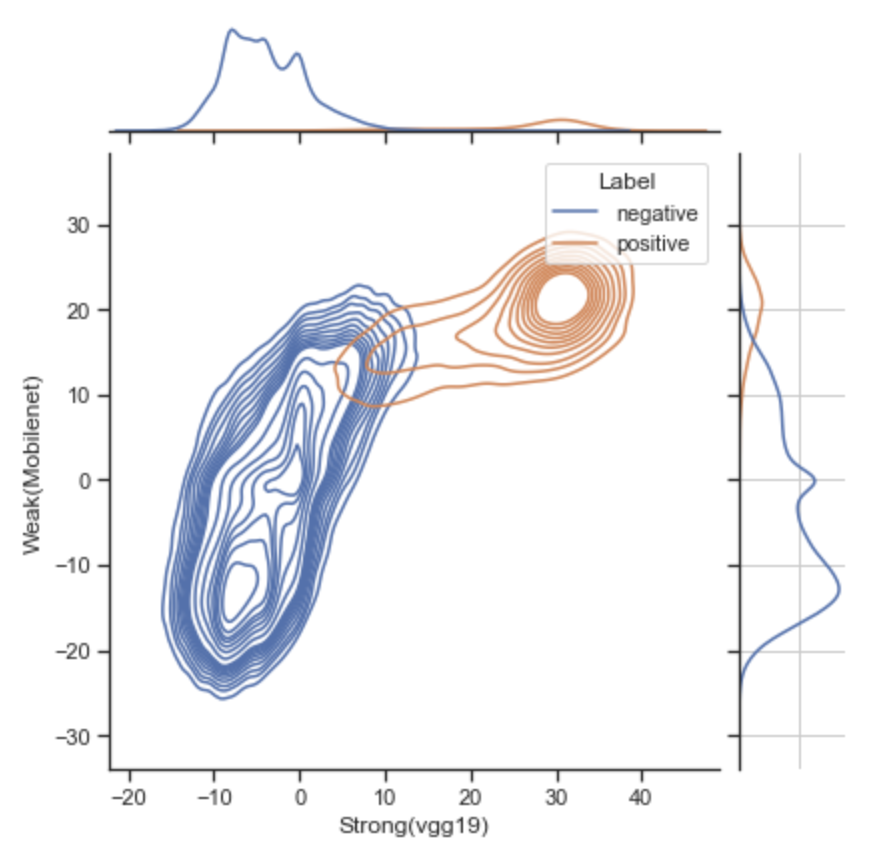
\includegraphics[width=2.5in]{figs/mobilenet_vgg_kde10_bs.png}}
    \subfigure[Ensemble Size=10, Random Start]{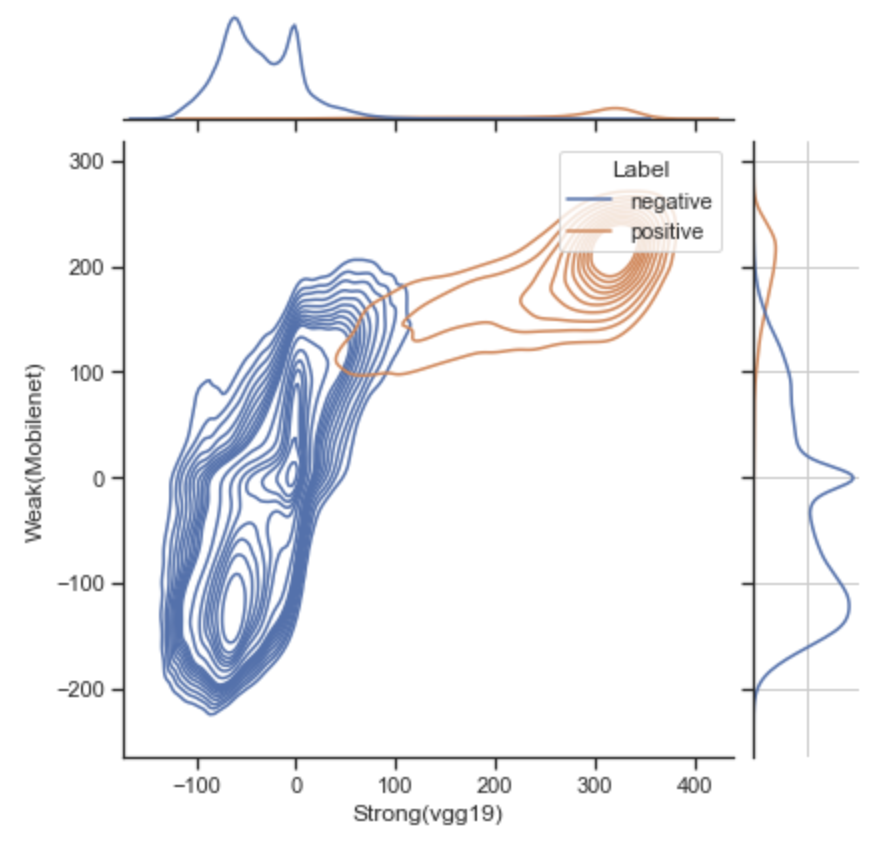
\includegraphics[width=2.5in]{figs/mobilenet_vgg_kde100_bs.png}}
    \quad 
    \subfigure[Ensemble Size=10, BootStrap]{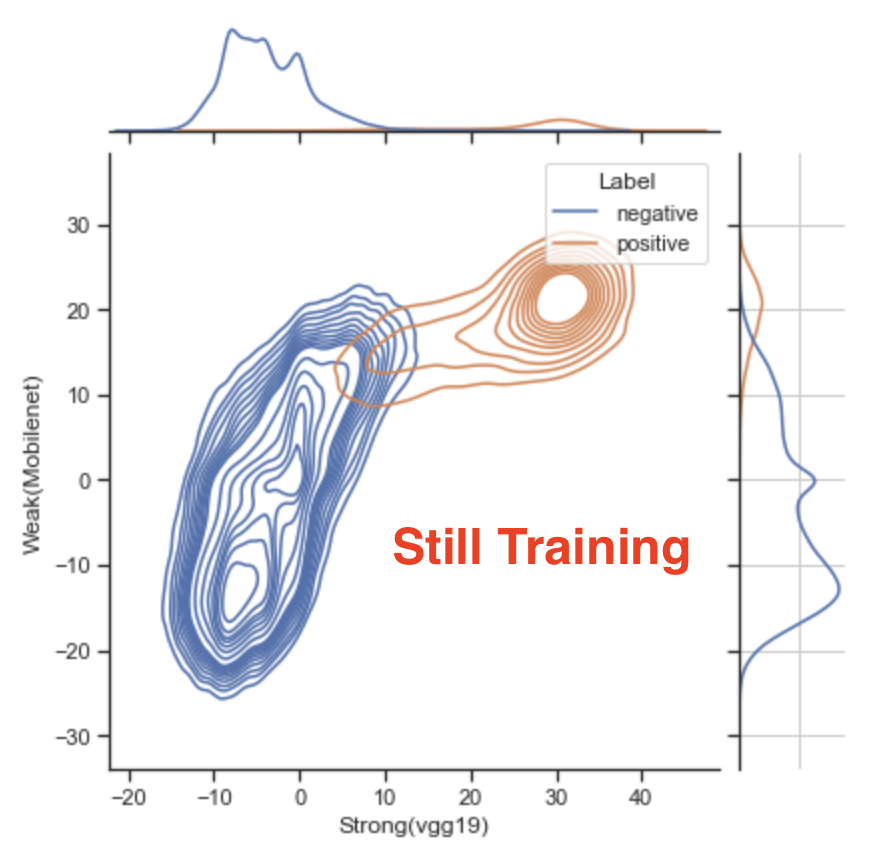
\includegraphics[width=2.5in]{figs/mobilenet_vgg_kde10_rsp.png}}
    \subfigure[Ensemble Size=100,BootStrap]{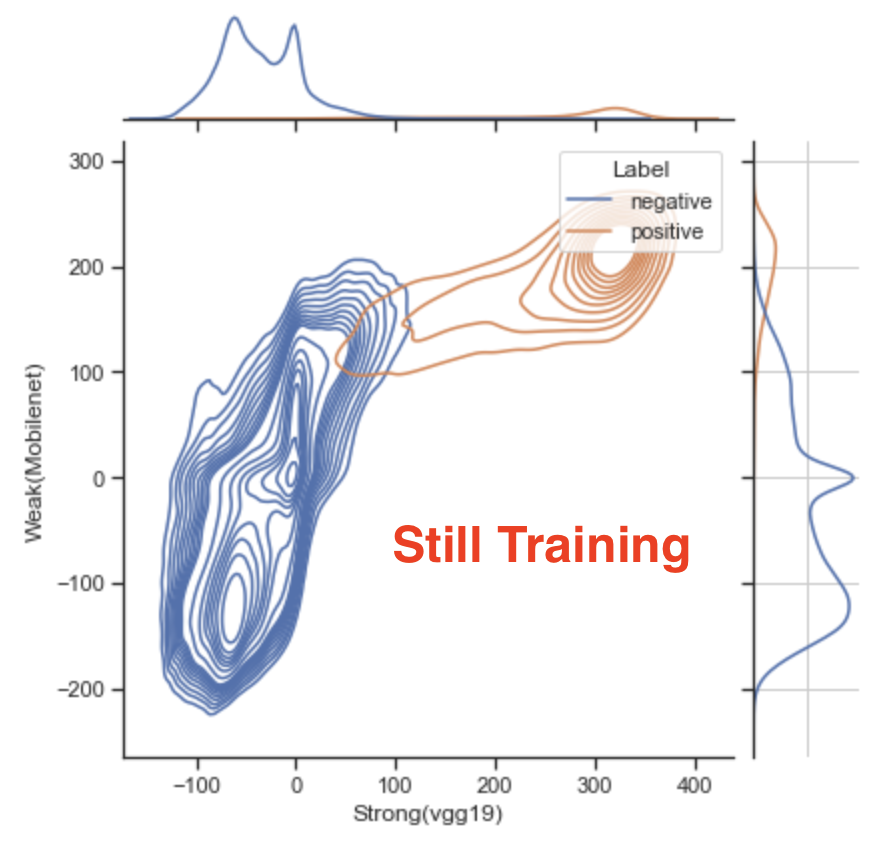
\includegraphics[width=2.5in]{figs/mobilenet_vgg_kde100_rsp.png}}
    \caption{\textbf{KDE Plot of Confidence of Strong and Weak Architectures}: The strong architecture is Vgg19, the weak architecture is MobileNet}
    \label{fig:kde_vgg_mobilenet}
\end{figure}


\subsection{Compare Human Results with Machine Results}
With our t-test based method, we can have different ways to combine the outputs of different architectures. Here we illustrate two ways and compare their results with human prediction. 

\subsubsection{Combination Way 1 }
Following the framework shown in \ref{fig:struc}, we use the 3rd way in section \ref{sec:multi} and only set a single threshold for each architecture and allow prediction sets rather than only a single class as the output. Then for each image, each architecture will give a prediction set. We regard every class in the set as getting one vote from the architecture. Combine the sets by all the architectures, we get a collection. In this collection, each class among the 10 will get zero or one or multiple votes from the architectures. Based on the frequencies of each class's votes, we can measure how likely it is for each class to be chosen as a final prediction. With CIFAR10H, we can compare the results of human labeler and our machine predictors. Figure \ref{fig:example_prob} illustrates some examples that human and machine have the same confusion.


\begin{figure}[H]
    \centering
    \subfigure[]{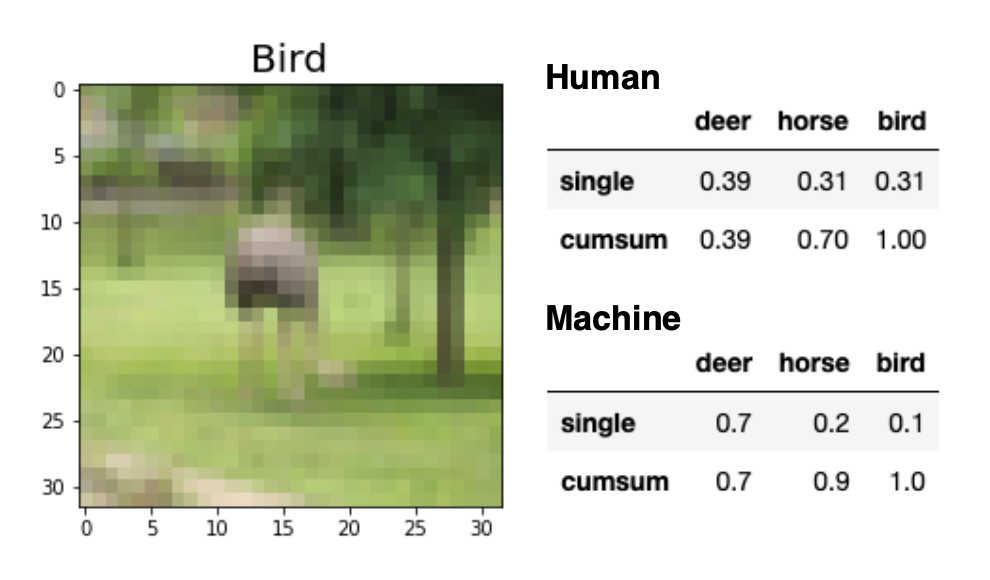
\includegraphics[scale=0.35]{figs/human_machine_agree_1.png}}
    \subfigure[]{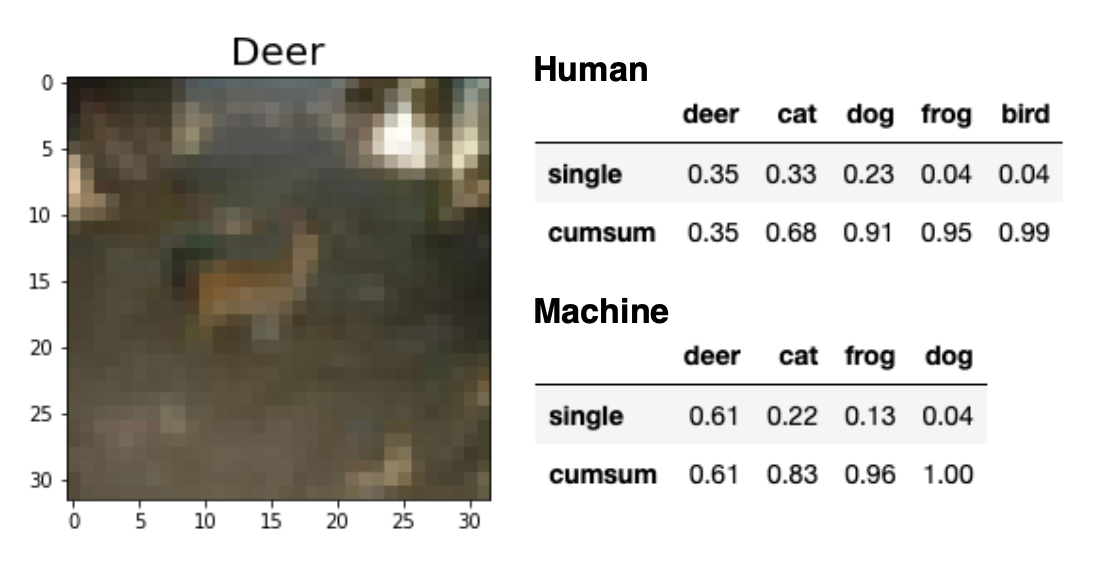
\includegraphics[scale=0.35]{figs/human_machine_agree_2.png}}
    \quad 
    \subfigure[]{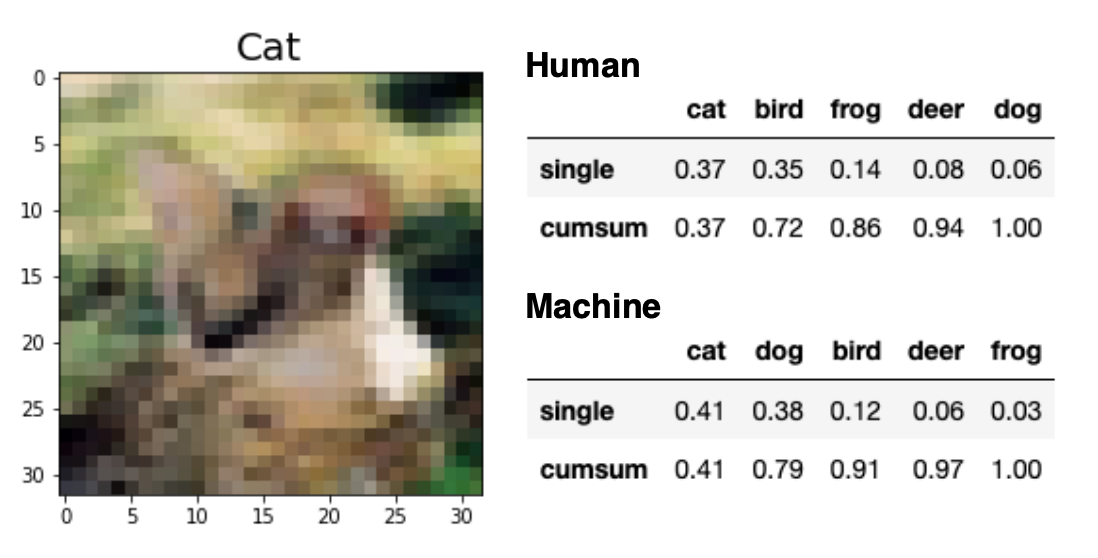
\includegraphics[scale=0.35]{figs/human_machine_agree_3.png}}
    \subfigure[]{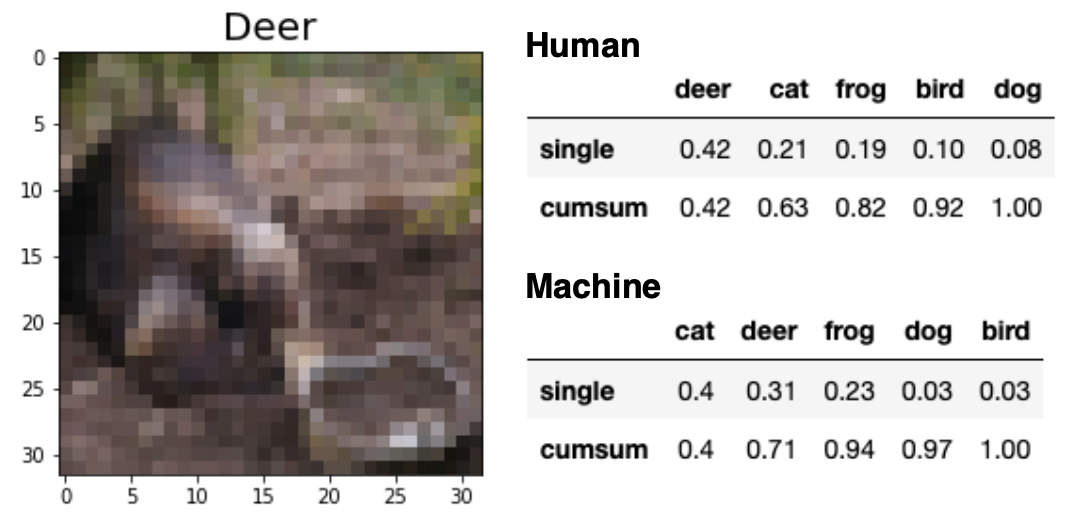
\includegraphics[scale=0.35]{figs/human_machine_agree_4.png}}
    \caption{\textbf{Examples That Human and Machine have the Same Confusion}: The tables shows the frequencies of votes of human labeler and machine predictors. The rows with index 'single' are the frequencies for each single class, the unshown classes all have zero frequencies. The rows with index 'cumsum' are the culmulative sum of the above row.}
    \label{fig:example_prob}
\end{figure}

For each image, we can use entropy of the frequency distribution by human/machine to measure how confusing it is for human/machine. We can use L1 distance between the frequency distributions by human and machine to measure their difference. We can denote each image as a point in the $\left[X,Y\right]$ plane where the $X$ axis is the machine entropy, and the $Y$ axis is the L1 distance between human and machine. A density plot is shown in Figure \ref{l1entropyscatter}

\begin{figure}[H]
    \centering
    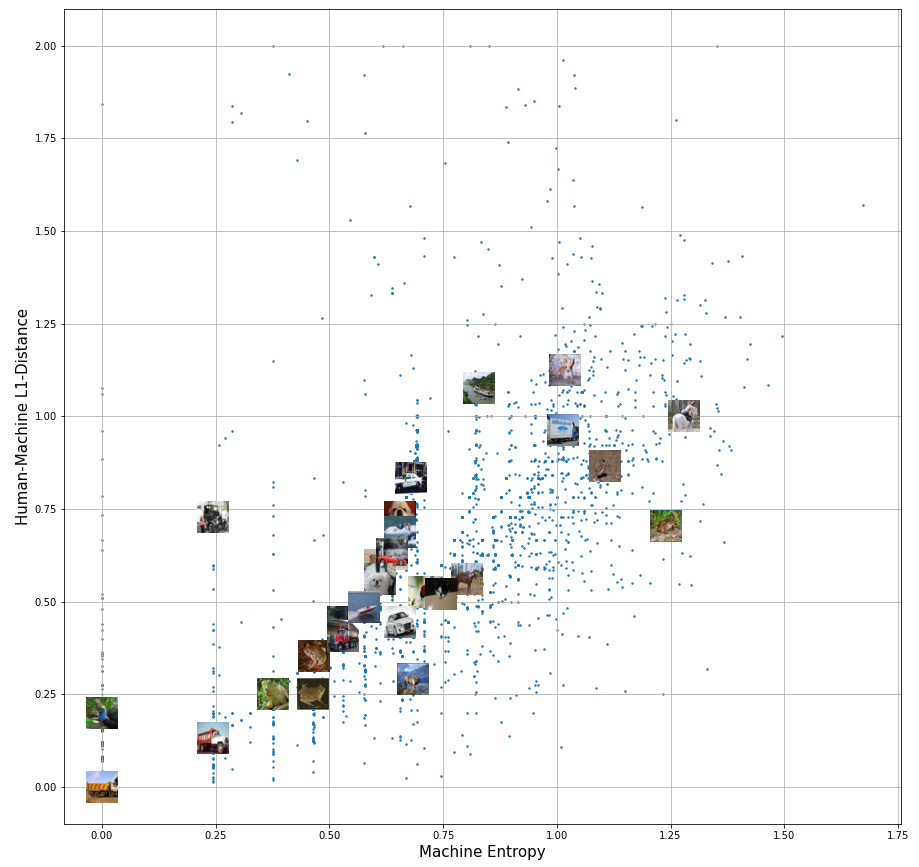
\includegraphics[scale=0.4]{figs/l1_entropy_scatter.png}
    \label{l1entropyscatter}
    \caption{\textbf{Entropy-L1 Scatter Plot}}
\end{figure}

\subsubsection{Combination Way 2}
Using the 3rd way in section \ref{sec:multi} and set two thresholds for each architecture to separate 'Confident Positive(+)', 'I don't know(0)', and 'Confident Negative(-)'. For each test instance, each class gets $K$ votes in ${+,0,-}$ from the $K$ architectures. If a class has more than $T$ votes of $+$ and 0 vote of $-$, then we say this class belong to the prediction set of this instance.

We compare the results of this combination way with the human results in the following way:
for a test instance, we have the machine generated prediction set and each class's  frequencies to be chosen by human. we first sum up the human frequencies of the classes in the prediction set to measure how much the machine results can match the human's judgements. Then we penalty large set size by minus the set size divided by the number of classes $C$. 

With this combination method. A prediction set whose size is 1 can get a score ranging from -0.1 to 0.9, size 2 can get -0.2 to 0.8 and size 3 from -0.3 to 0.7. Figure\ref{fig:cdf_score} and Figure\ref{fig:human_machine_example} shows the culmulative distribution function of the distribution of this score under different set sizes.


\begin{figure}[H]
    \centering
    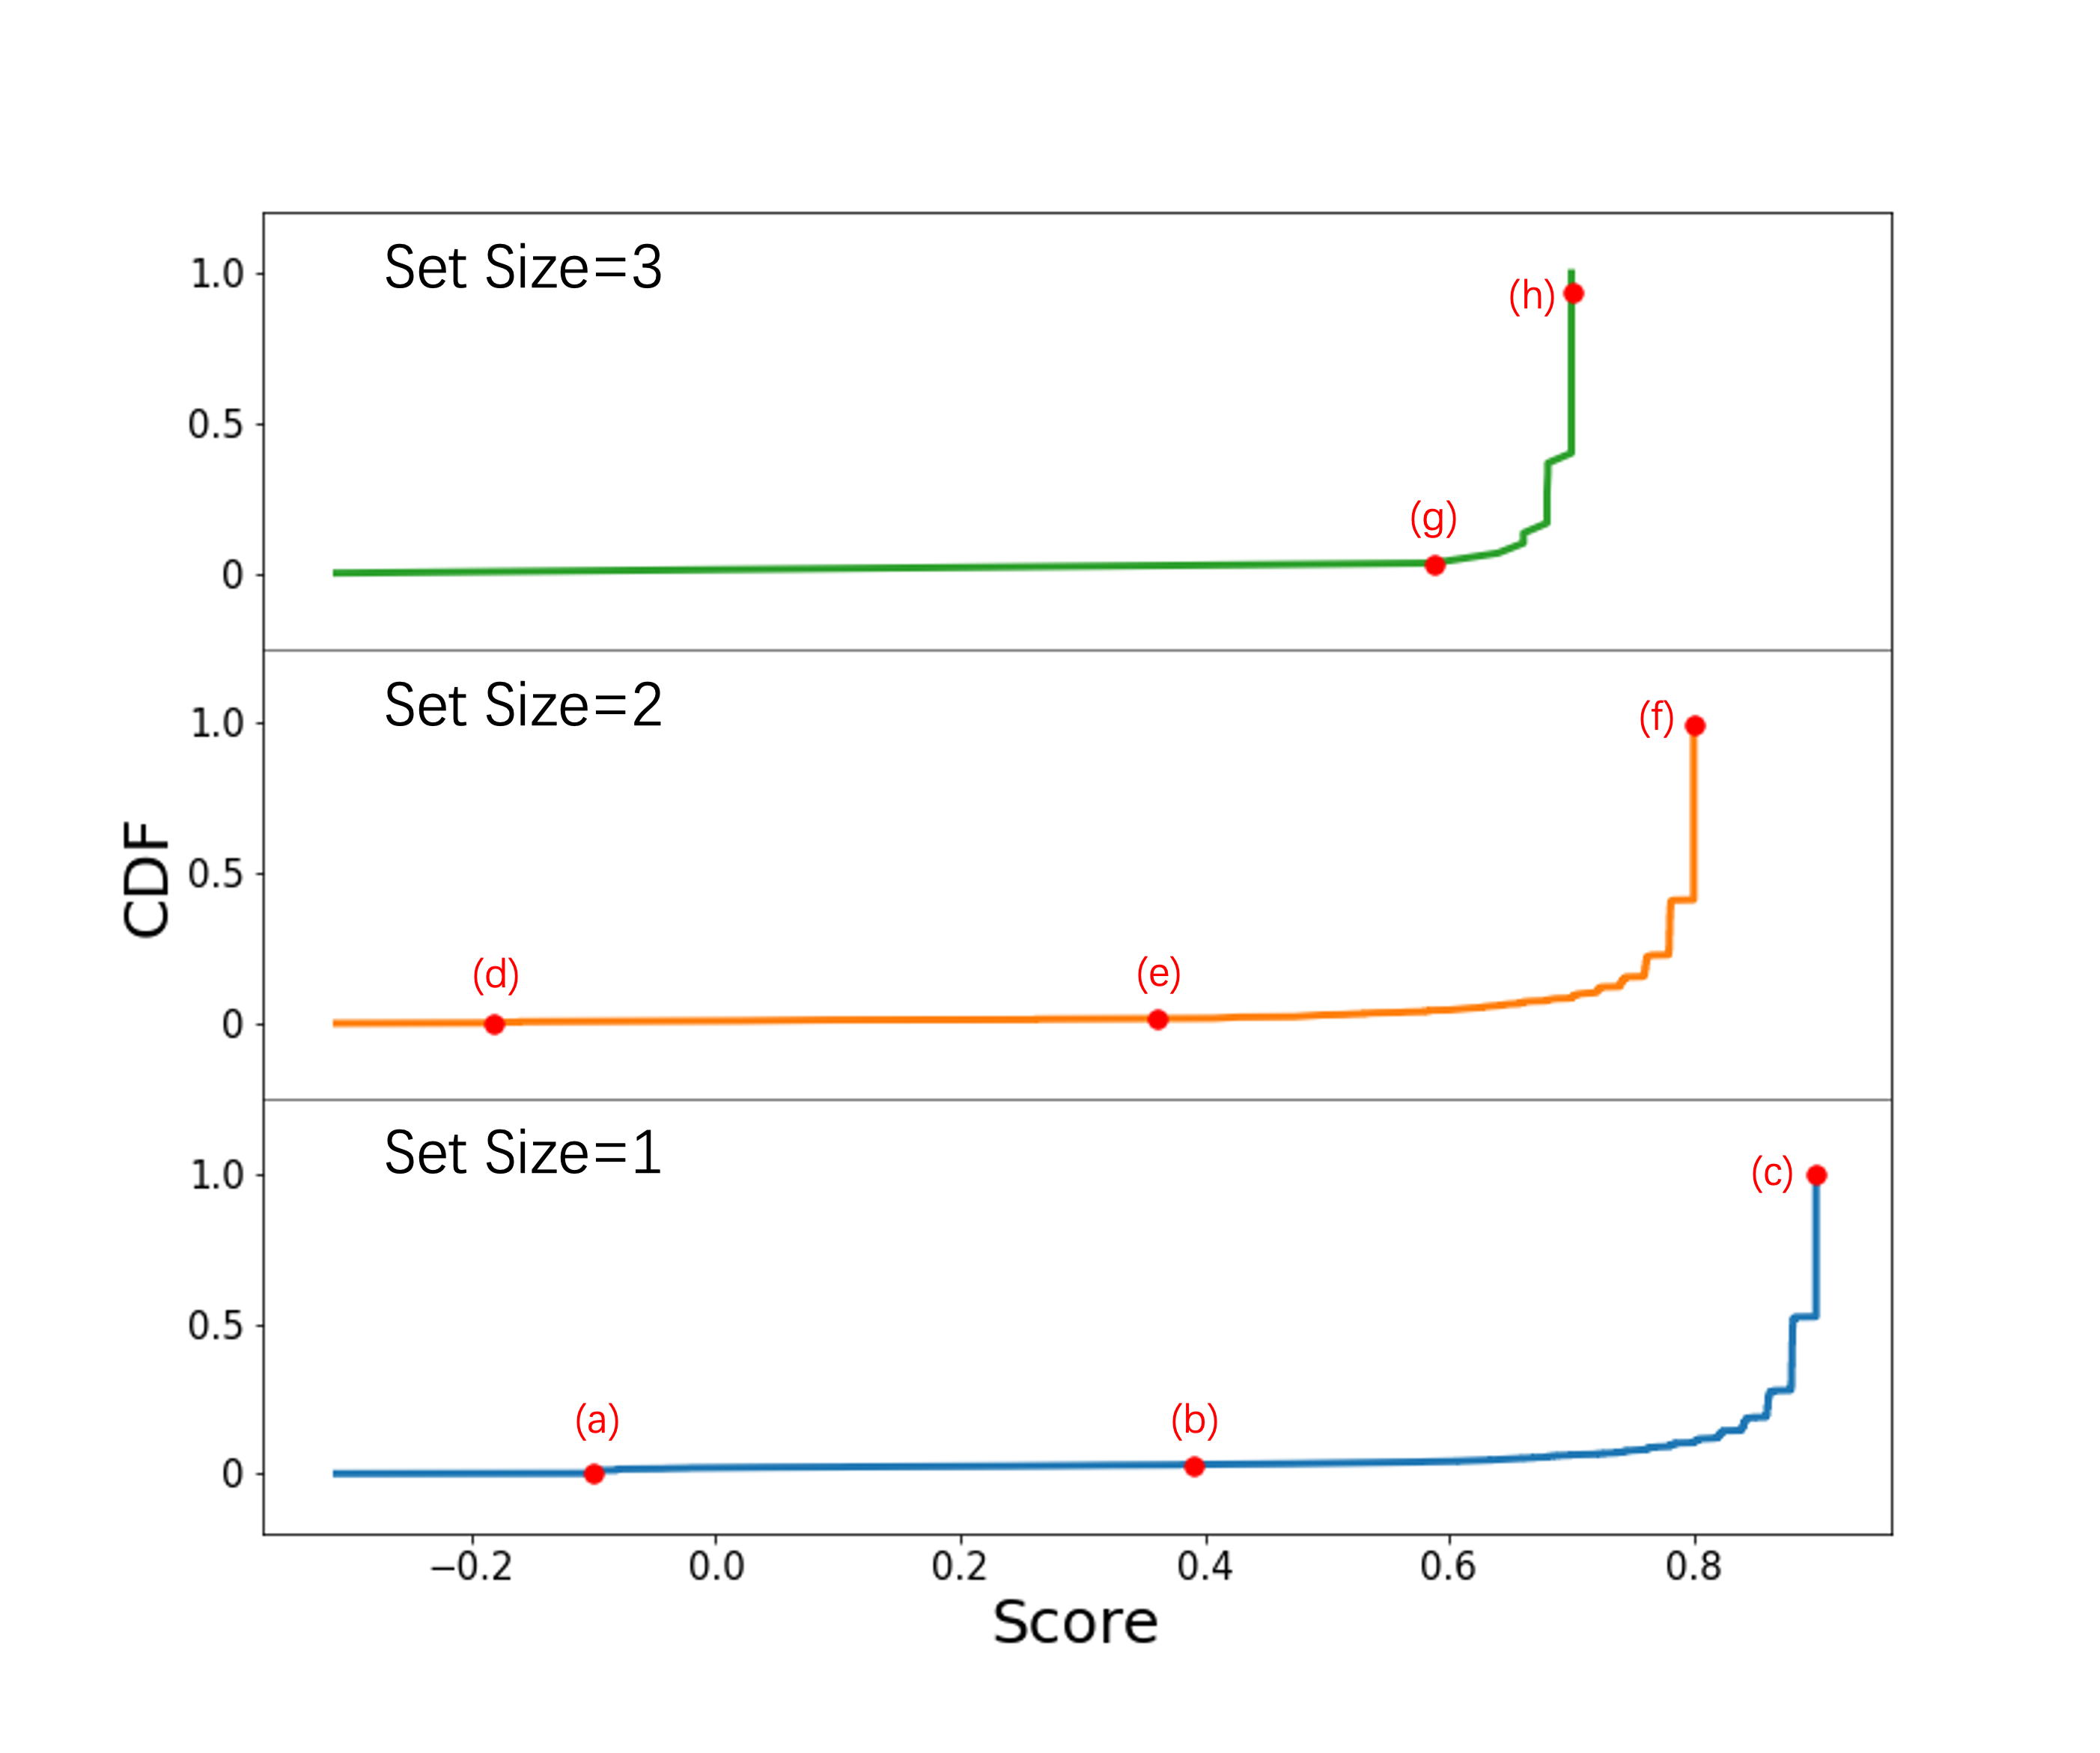
\includegraphics[scale=0.6]{figs/cdf_score_full.png}
    \label{cdf_score}
    \caption{\textbf{CDF of The Score for Different Set Sizes} To choose the 2 thresholds to separate $+,0,-$, we first get the culmulative distribution function(CDF) of positive binary instances and complementary culmulative distribution function(CCDF) of negative binary instances. Set the confidence score where negative CCDF value = 10\% and the score where positive CDF value=90\% as the 2 thresholds. $T=1$, which is the least thresholds of $+$ votes.}
\end{figure}


\begin{figure}[H]
    \centering
    \hspace{-10mm}
    \subfigure[]{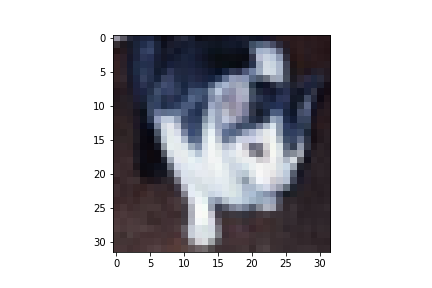
\includegraphics[scale=0.35]{figs/new_comb_fig/1_3594.png} \label{subfig:a}}
    \hspace{-24mm}
    \subfigure[]{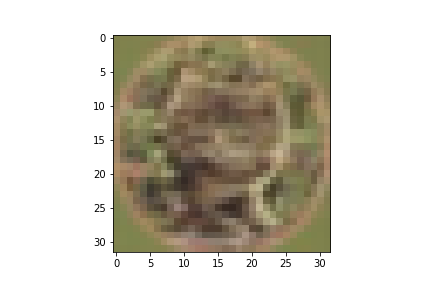
\includegraphics[scale=0.35]{figs/new_comb_fig/1_5511.png}}
    \hspace{-24mm}
    \subfigure[]{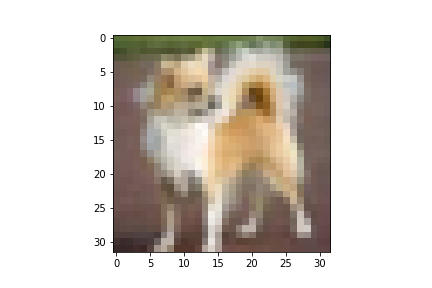
\includegraphics[scale=0.35]{figs/new_comb_fig/1_5035.png}}
    \hspace{-24mm}
    \subfigure[]{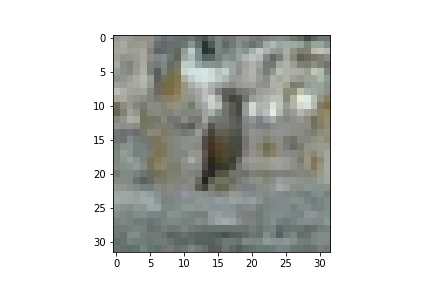
\includegraphics[scale=0.35]{figs/new_comb_fig/2_2270.png}}

    \hspace{-10mm}
    \subfigure[]{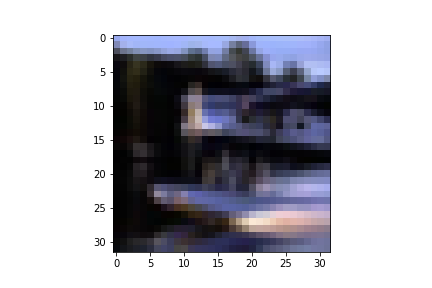
\includegraphics[scale=0.35]{figs/new_comb_fig/2_3211.png}}
    \hspace{-24mm}
    \subfigure[]{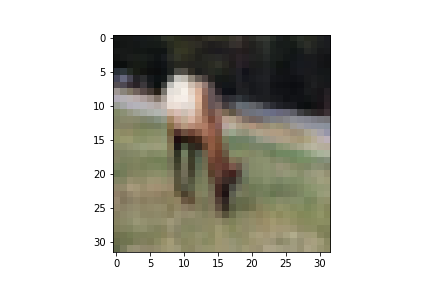
\includegraphics[scale=0.35]{figs/new_comb_fig/2_3962.png}}
    \hspace{-24mm}
    \subfigure[]{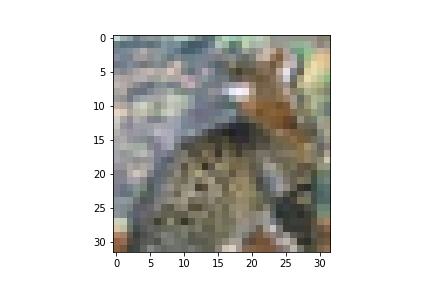
\includegraphics[scale=0.35]{figs/new_comb_fig/3_9497.png}}
    \hspace{-24mm}
    \subfigure[]{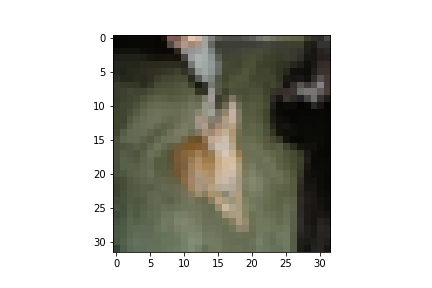
\includegraphics[scale=0.35]{figs/new_comb_fig/3_470.png}}
    \caption{\textbf{Examples of Human and Machine Classification} (a)\textbf{Human}: Cat(1.0). \textbf{Machine}: Dog. (b)\textbf{Human}: Frog(0.49), Cat(0.47), Bird(0.04). \textbf{Machine}: Frog. (c)\textbf{Human}: Dog(1.0). \textbf{Machine}: Dog. (d)\textbf{Human}: Bird(0.92), Ship(0.02), Frog(0.02), Dog(0.02), Cat(0.02). \textbf{Machine}: Cat, Dear. (e)\textbf{Human}: Airplane(0.56), Ship(0.44). \textbf{Machine}: Truck, Airplane. (f)\textbf{Human}: Deer(0.6), Horse(0.4). \textbf{Machine}: Deer, Horse. (g)\textbf{Human}: Cat(0.72), Frog(0.09), Deer(0.09), Bird(0.08), Airplane(0.02). \textbf{Machine}: Cat, Frog, Bird. (h)\textbf{Human}: Cat(0.65), Dog(0.21), Deer(0.14). \textbf{Machine}: Dog, Deer, Cat} 
    \label{fig:human_machine_example}
\end{figure}



\subsection{Example: Weak-Strong Flow}
To see how the above finds can be applied, we establish a weak-strong flow where we consturct an ensemble with a weak yet fast architecture and another ensemble with a strong yet slow architecture. For each coming image, the weak ensemble labels $+$, $-$, or $0$ for each class using the 3rd way in section \ref{sec:multi} with two thresholds, where $+$ represents being confident of belonging to this class, $-$ for confident of not belonging to this class, or $0$ for "I don't know" . If there is only one class with the label $+$, then this class will be the final result. Otherwise we call the strong the strong ensemble and make a prediction with the 1st way in section \ref{sec:multi}. 

The accuracy of this weak-strong flow is 0000. To compare, the accuracy for purly running an easy ensemble with the 1st way in section \ref{sec:multi} is 00000. The accuracy of running the strong ensemble only is 0000000

Table \ref{WSFlow} and \ref{strong_only} show the running time of the weak-strong flow and only running the strong ensemble.


\begin{table}
    \caption{\textbf{Running Time of Weak-Strong Flow}: The weak model is MobileNet, the strong model is DPN92, the ensemble size for both architectures are 10. Batch Size indicates how how many images are processed parallelly by the weak-strong flow. The unit for all values is ms.}
    \centering
    \begin{tabular}{crrrrr}
        \toprule
        {} Batch Size &  Weak Run &  Weak T-Test &  Strong Run &  Strong T-Test &  Weak-Strong Flow Total \\
        % Batch Size &           &              &             &                &                         \\
        \midrule
        16         &   0.54016 &      0.04063 &     3.38590 &        0.03598 &                 4.00267 \\
        64         &   0.32618 &      0.01138 &     2.32941 &        0.00957 &                 2.67653 \\
        256        &   0.42272 &      0.00420 &     2.83185 &        0.00308 &                 3.26185 \\
        1024       &   0.33215 &      0.00329 &     2.68724 &        0.00153 &                 3.02421 \\
        \bottomrule
    \end{tabular}
\label{WSFlow}
\end{table}

\begin{table}
    \caption{\textbf{Running Time of the Strong Ensemble Only}: The strong model is DPN92, the ensemble size is 10. Batch Size indicates how how many images are processed parallelly. The unit for all values is ms}
    \centering
    \begin{tabular}{crrr}
        \toprule
        {} Batch Size &  Strong Only Run &  Strong Only T-Test &  Strong Only Total \\
        % Batch Size &                  &                     &                    \\
        \midrule
        16         &          5.93767 &             0.03345 &            5.97112 \\
        64         &          4.93924 &             0.00943 &            4.94867 \\
        256        &          5.70755 &             0.00375 &            5.71130 \\
        1024       &          7.01784 &             0.00224 &            7.02008 \\
        \bottomrule
        \end{tabular}
\label{strong_only}
\end{table}

% \section{Submission of papers to NeurIPS 2023}


% Please read the instructions below carefully and follow them faithfully.


% \subsection{Style}


% Papers to be submitted to NeurIPS 2023 must be prepared according to the
% instructions presented here. Papers may only be up to {\bf nine} pages long,
% including figures. Additional pages \emph{containing only acknowledgments and
% references} are allowed. Papers that exceed the page limit will not be
% reviewed, or in any other way considered for presentation at the conference.


% The margins in 2023 are the same as those in previous years.


% Authors are required to use the NeurIPS \LaTeX{} style files obtainable at the
% NeurIPS website as indicated below. Please make sure you use the current files
% and not previous versions. Tweaking the style files may be grounds for
% rejection.


% \subsection{Retrieval of style files}


% The style files for NeurIPS and other conference information are available on
% the website at
% \begin{center}
%   \url{http://www.neurips.cc/}
% \end{center}
% The file \verb+neurips_2023.pdf+ contains these instructions and illustrates the
% various formatting requirements your NeurIPS paper must satisfy.


% The only supported style file for NeurIPS 2023 is \verb+neurips_2023.sty+,
% rewritten for \LaTeXe{}.  \textbf{Previous style files for \LaTeX{} 2.09,
%   Microsoft Word, and RTF are no longer supported!}


% The \LaTeX{} style file contains three optional arguments: \verb+final+, which
% creates a camera-ready copy, \verb+preprint+, which creates a preprint for
% submission to, e.g., arXiv, and \verb+nonatbib+, which will not load the
% \verb+natbib+ package for you in case of package clash.


% \paragraph{Preprint option}
% If you wish to post a preprint of your work online, e.g., on arXiv, using the
% NeurIPS style, please use the \verb+preprint+ option. This will create a
% nonanonymized version of your work with the text ``Preprint. Work in progress.''
% in the footer. This version may be distributed as you see fit, as long as you do not say which conference it was submitted to. Please \textbf{do
%   not} use the \verb+final+ option, which should \textbf{only} be used for
% papers accepted to NeurIPS. 


% At submission time, please omit the \verb+final+ and \verb+preprint+
% options. This will anonymize your submission and add line numbers to aid
% review. Please do \emph{not} refer to these line numbers in your paper as they
% will be removed during generation of camera-ready copies.


% The file \verb+neurips_2023.tex+ may be used as a ``shell'' for writing your
% paper. All you have to do is replace the author, title, abstract, and text of
% the paper with your own.


% The formatting instructions contained in these style files are summarized in
% Sections \ref{gen_inst}, \ref{headings}, and \ref{others} below.


% \section{General formatting instructions}
% \label{gen_inst}


% The text must be confined within a rectangle 5.5~inches (33~picas) wide and
% 9~inches (54~picas) long. The left margin is 1.5~inch (9~picas).  Use 10~point
% type with a vertical spacing (leading) of 11~points.  Times New Roman is the
% preferred typeface throughout, and will be selected for you by default.
% Paragraphs are separated by \nicefrac{1}{2}~line space (5.5 points), with no
% indentation.


% The paper title should be 17~point, initial caps/lower case, bold, centered
% between two horizontal rules. The top rule should be 4~points thick and the
% bottom rule should be 1~point thick. Allow \nicefrac{1}{4}~inch space above and
% below the title to rules. All pages should start at 1~inch (6~picas) from the
% top of the page.


% For the final version, authors' names are set in boldface, and each name is
% centered above the corresponding address. The lead author's name is to be listed
% first (left-most), and the co-authors' names (if different address) are set to
% follow. If there is only one co-author, list both author and co-author side by
% side.


% Please pay special attention to the instructions in Section \ref{others}
% regarding figures, tables, acknowledgments, and references.


% \section{Headings: first level}
% \label{headings}


% All headings should be lower case (except for first word and proper nouns),
% flush left, and bold.


% First-level headings should be in 12-point type.


% \subsection{Headings: second level}


% Second-level headings should be in 10-point type.


% \subsubsection{Headings: third level}


% Third-level headings should be in 10-point type.


% \paragraph{Paragraphs}


% There is also a \verb+\paragraph+ command available, which sets the heading in
% bold, flush left, and inline with the text, with the heading followed by 1\,em
% of space.


% \section{Citations, figures, tables, references}
% \label{others}


% These instructions apply to everyone.


% \subsection{Citations within the text}


% The \verb+natbib+ package will be loaded for you by default.  Citations may be
% author/year or numeric, as long as you maintain internal consistency.  As to the
% format of the references themselves, any style is acceptable as long as it is
% used consistently.


% The documentation for \verb+natbib+ may be found at
% \begin{center}
%   \url{http://mirrors.ctan.org/macros/latex/contrib/natbib/natnotes.pdf}
% \end{center}
% Of note is the command \verb+\citet+, which produces citations appropriate for
% use in inline text.  For example,
% \begin{verbatim}
%    \citet{hasselmo} investigated\dots
% \end{verbatim}
% produces
% \begin{quote}
%   Hasselmo, et al.\ (1995) investigated\dots
% \end{quote}


% If you wish to load the \verb+natbib+ package with options, you may add the
% following before loading the \verb+neurips_2023+ package:
% \begin{verbatim}
%    \PassOptionsToPackage{options}{natbib}
% \end{verbatim}


% If \verb+natbib+ clashes with another package you load, you can add the optional
% argument \verb+nonatbib+ when loading the style file:
% \begin{verbatim}
%    \usepackage[nonatbib]{neurips_2023}
% \end{verbatim}


% As submission is double blind, refer to your own published work in the third
% person. That is, use ``In the previous work of Jones et al.\ [4],'' not ``In our
% previous work [4].'' If you cite your other papers that are not widely available
% (e.g., a journal paper under review), use anonymous author names in the
% citation, e.g., an author of the form ``A.\ Anonymous'' and include a copy of the anonymized paper in the supplementary material.


% \subsection{Footnotes}


% Footnotes should be used sparingly.  If you do require a footnote, indicate
% footnotes with a number\footnote{Sample of the first footnote.} in the
% text. Place the footnotes at the bottom of the page on which they appear.
% Precede the footnote with a horizontal rule of 2~inches (12~picas).


% Note that footnotes are properly typeset \emph{after} punctuation
% marks.\footnote{As in this example.}


% \subsection{Figures}


% \begin{figure}
%   \centering
%   \fbox{\rule[-.5cm]{0cm}{4cm} \rule[-.5cm]{4cm}{0cm}}
%   \caption{Sample figure caption.}
% \end{figure}


% All artwork must be neat, clean, and legible. Lines should be dark enough for
% purposes of reproduction. The figure number and caption always appear after the
% figure. Place one line space before the figure caption and one line space after
% the figure. The figure caption should be lower case (except for first word and
% proper nouns); figures are numbered consecutively.


% You may use color figures.  However, it is best for the figure captions and the
% paper body to be legible if the paper is printed in either black/white or in
% color.


% \subsection{Tables}


% All tables must be centered, neat, clean and legible.  The table number and
% title always appear before the table.  See Table~\ref{sample-table}.


% Place one line space before the table title, one line space after the
% table title, and one line space after the table. The table title must
% be lower case (except for first word and proper nouns); tables are
% numbered consecutively.


% Note that publication-quality tables \emph{do not contain vertical rules.} We
% strongly suggest the use of the \verb+booktabs+ package, which allows for
% typesetting high-quality, professional tables:
% \begin{center}
%   \url{https://www.ctan.org/pkg/booktabs}
% \end{center}
% This package was used to typeset Table~\ref{sample-table}.


% \begin{table}
%   \caption{Sample table title}
%   \label{sample-table}
%   \centering
%   \begin{tabular}{lll}
%     \toprule
%     \multicolumn{2}{c}{Part}                   \\
%     \cmidrule(r){1-2}
%     Name     & Description     & Size ($\mu$m) \\
%     \midrule
%     Dendrite & Input terminal  & $\sim$100     \\
%     Axon     & Output terminal & $\sim$10      \\
%     Soma     & Cell body       & up to $10^6$  \\
%     \bottomrule
%   \end{tabular}
% \end{table}

% \subsection{Math}
% Note that display math in bare TeX commands will not create correct line numbers for submission. Please use LaTeX (or AMSTeX) commands for unnumbered display math. (You really shouldn't be using \$\$ anyway; see \url{https://tex.stackexchange.com/questions/503/why-is-preferable-to} and \url{https://tex.stackexchange.com/questions/40492/what-are-the-differences-between-align-equation-and-displaymath} for more information.)

% \subsection{Final instructions}

% Do not change any aspects of the formatting parameters in the style files.  In
% particular, do not modify the width or length of the rectangle the text should
% fit into, and do not change font sizes (except perhaps in the
% \textbf{References} section; see below). Please note that pages should be
% numbered.


% \section{Preparing PDF files}


% Please prepare submission files with paper size ``US Letter,'' and not, for
% example, ``A4.''


% Fonts were the main cause of problems in the past years. Your PDF file must only
% contain Type 1 or Embedded TrueType fonts. Here are a few instructions to
% achieve this.


% \begin{itemize}


% \item You should directly generate PDF files using \verb+pdflatex+.


% \item You can check which fonts a PDF files uses.  In Acrobat Reader, select the
%   menu Files$>$Document Properties$>$Fonts and select Show All Fonts. You can
%   also use the program \verb+pdffonts+ which comes with \verb+xpdf+ and is
%   available out-of-the-box on most Linux machines.


% \item \verb+xfig+ "patterned" shapes are implemented with bitmap fonts.  Use
%   "solid" shapes instead.


% \item The \verb+\bbold+ package almost always uses bitmap fonts.  You should use
%   the equivalent AMS Fonts:
% \begin{verbatim}
%    \usepackage{amsfonts}
% \end{verbatim}
% followed by, e.g., \verb+\mathbb{R}+, \verb+\mathbb{N}+, or \verb+\mathbb{C}+
% for $\mathbb{R}$, $\mathbb{N}$ or $\mathbb{C}$.  You can also use the following
% workaround for reals, natural and complex:
% \begin{verbatim}
%    \newcommand{\RR}{I\!\!R} %real numbers
%    \newcommand{\Nat}{I\!\!N} %natural numbers
%    \newcommand{\CC}{I\!\!\!\!C} %complex numbers
% \end{verbatim}
% Note that \verb+amsfonts+ is automatically loaded by the \verb+amssymb+ package.


% \end{itemize}


% If your file contains type 3 fonts or non embedded TrueType fonts, we will ask
% you to fix it.


% \subsection{Margins in \LaTeX{}}


% Most of the margin problems come from figures positioned by hand using
% \verb+\special+ or other commands. We suggest using the command
% \verb+\includegraphics+ from the \verb+graphicx+ package. Always specify the
% figure width as a multiple of the line width as in the example below:
% \begin{verbatim}
%    \usepackage[pdftex]{graphicx} ...
%    \includegraphics[width=0.8\linewidth]{myfile.pdf}
% \end{verbatim}
% See Section 4.4 in the graphics bundle documentation
% (\url{http://mirrors.ctan.org/macros/latex/required/graphics/grfguide.pdf})


% A number of width problems arise when \LaTeX{} cannot properly hyphenate a
% line. Please give LaTeX hyphenation hints using the \verb+\-+ command when
% necessary.


% \begin{ack}
% Use unnumbered first level headings for the acknowledgments. All acknowledgments
% go at the end of the paper before the list of references. Moreover, you are required to declare
% funding (financial activities supporting the submitted work) and competing interests (related financial activities outside the submitted work).
% More information about this disclosure can be found at: \url{https://neurips.cc/Conferences/2023/PaperInformation/FundingDisclosure}.


% Do {\bf not} include this section in the anonymized submission, only in the final paper. You can use the \texttt{ack} environment provided in the style file to autmoatically hide this section in the anonymized submission.
% \end{ack}



% \section{Supplementary Material}

% Authors may wish to optionally include extra information (complete proofs, additional experiments and plots) in the appendix. All such materials should be part of the supplemental material (submitted separately) and should NOT be included in the main submission.


% \section*{References Original}


% References follow the acknowledgments in the camera-ready paper. Use unnumbered first-level heading for
% the references. Any choice of citation style is acceptable as long as you are
% consistent. It is permissible to reduce the font size to \verb+small+ (9 point)
% when listing the references.
% Note that the Reference section does not count towards the page limit.
% \medskip


% {
% \small


% [1] Alexander, J.A.\ \& Mozer, M.C.\ (1995) Template-based algorithms for
% connectionist rule extraction. In G.\ Tesauro, D.S.\ Touretzky and T.K.\ Leen
% (eds.), {\it Advances in Neural Information Processing Systems 7},
% pp.\ 609--616. Cambridge, MA: MIT Press.


% [2] Bower, J.M.\ \& Beeman, D.\ (1995) {\it The Book of GENESIS: Exploring
%   Realistic Neural Models with the GEneral NEural SImulation System.}  New York:
% TELOS/Springer--Verlag.


% [3] Hasselmo, M.E., Schnell, E.\ \& Barkai, E.\ (1995) Dynamics of learning and
% recall at excitatory recurrent synapses and cholinergic modulation in rat
% hippocampal region CA3. {\it Journal of Neuroscience} {\bf 15}(7):5249-5262.
% }

%%%%%%%%%%%%%%%%%%%%%%%%%%%%%%%%%%%%%%%%%%%%%%%%%%%%%%%%%%%%
\bibliographystyle{plain}
\bibliography{refs.bib}
\end{document}
%%% Local Variables:
%%% mode: latex
%%% TeX-master: t
%%% End:
